\section{Einschaltvorgang}
Beim Einschaltvorgang wird der Stromverlauf aller Stränge mit einem Oszilloskop gemessen (siehe Abbildung\;\ref{fig:Einschaltvorgang_Messschaltung}).
\begin{figure}
    \centering
    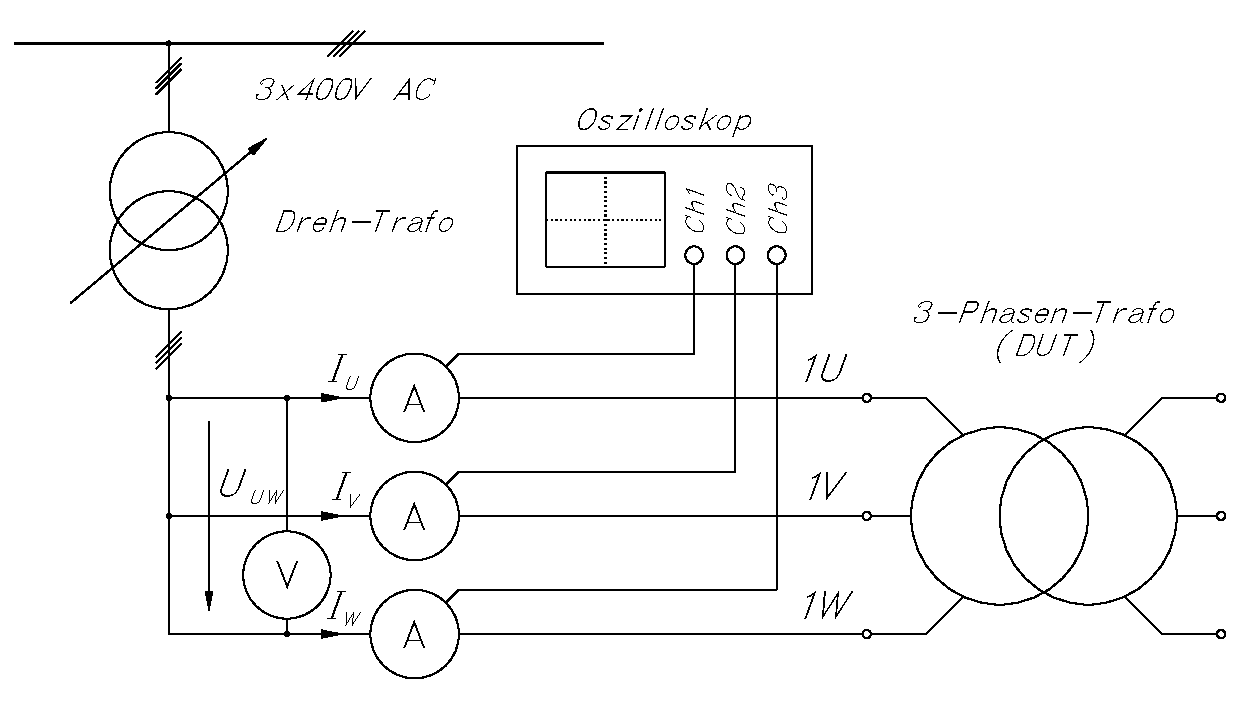
\includegraphics[width=0.75\textwidth, angle=0]{2/images/Einschaltversuch.pdf}
    \caption{Messschaltung für die Erfassung der primärseitigen Strangströme (=Aussenleiterströme) $I_U, I_V, I_W$ mittels Stromzangen und Oszilloskop.}
    \label{fig:Einschaltvorgang_Messschaltung}
\end{figure}\\
\noindent Der Transformator wird schlagartig ans Netz geschaltet. Der Betrag der mit dem Einschwingvorgang einhergehenden Ströme hängt dabei stark vom Einschaltzeitpunkt ab.\\
Unmittelbar nach dem Einschalten stellt sich ein magnetischer Fluss ein, der proportional der Spannungszeitfläche ist. Erfolgt das Einschalten genau bei einem Nulldurchgang der Netzspannung, entsteht der größtmögliche Fluss. Dies entspricht genau dem zweifachen Spitzenwert des stationären Flusses. Die so entstehenden Flussspitzen führen aufgrund der Sättigung des Trafoblechs zu stark verzerrten Strömen mit Spitzenwerten von bis zu 15-fachem Nennstrom. Dieser nichtlineare Zussammenhang ist über die Magnetisierungskennlinie gegeben. In Abbildung \ref{fig:Einschaltvorgang_worstcase} ist ein Einschwingvorgang mit einem hohem Strom dargestellt. Das Betragsmaximum von $I_U$ liegt bei $\SI{648}{\ampere}$, was etwa $853\%$ des Nennstromes entspricht.

\input{\currfiledir worstcase}

\noindent Der ideale Einschaltzeitpunkt liegt bei einem Maximum der Versorgungsspannung und resultiert in keiner Stromüberhöhung. In Abbildung \ref{fig:Einschaltvorgang_bestcase}) ist ein Einschwingvorgang mit niedrigerem Einschaltstrom dargestellt. Das Betragsmaximum von $I_V$ liegt bei $\SI{176}{\ampere}$, was nur mehr $232\%$ des Nennstromes entspricht.

\input{\currfiledir bestcase}
\clearpage